\documentclass[11pt,letterpaper]{article}

\usepackage{newtxtext,newtxmath}
\usepackage{microtype}
\usepackage[margin=1.25in]{geometry}
\usepackage{tikz}
\usetikzlibrary{arrows.meta,positioning,shapes.geometric,fit,backgrounds,calc}
\usepackage{booktabs}
\usepackage{listings}
\usepackage{xcolor}
\usepackage[colorlinks=true,linkcolor=black,urlcolor=black,citecolor=black]{hyperref}

\title{\textbf{AI Image Generation Pipeline}\\[0.5em]\large System Architecture}
\author{Srið{}ar Ayengar}
\date{\today}

\tikzset{
  component/.style={rectangle,rounded corners=3pt,draw=black,thick,fill=gray!10,
    minimum width=2.4cm,minimum height=0.7cm,font=\small\ttfamily,text centered},
  queue/.style={rectangle,draw=black,thick,fill=white,
    minimum width=2.4cm,minimum height=0.6cm,font=\small\ttfamily,text centered},
  exchange/.style={diamond,draw=black,thick,fill=gray!20,
    minimum width=2.2cm,minimum height=0.7cm,font=\small\ttfamily,text centered,aspect=2.5},
  store/.style={cylinder,draw=black,thick,fill=gray!15,shape border rotate=90,
    minimum width=1.8cm,minimum height=0.8cm,font=\small\ttfamily,text centered},
  arrow/.style={->,>=Stealth,thick},
  lbl/.style={font=\footnotesize\ttfamily,midway}
}

\begin{document}

\maketitle
\tableofcontents
\newpage

\section{Overview}

The AI image generation pipeline is an autonomous system that accepts a
natural language prompt and iteratively generates, scores, and refines
images until a candidate meeting all quality thresholds is accepted by a
tactical large language model (LLM).

The pipeline is designed around three principles:

\begin{enumerate}
  \item \textbf{Observable}: every message, score, and verdict flows through
        inspectable queues and addresses. Artemis's management console
        provides real-time visibility into all message flows. Dead-letter
        messages accumulate in \texttt{pipeline.dead} for operator review.
  \item \textbf{Scalable}: each component is independently deployable. The
        message broker provides natural decoupling. Adding scorer capacity
        requires only adding subscriber processes.
  \item \textbf{Persistent}: every generated image is recorded in LanceDB as
        a vector embedding alongside full scorer results and generation
        parameters. This long-term memory enables the strategic LLM to
        identify patterns across sessions.
\end{enumerate}

\section{Technology Stack}

\begin{center}
\begin{tabular}{lll}
\toprule
\textbf{Layer} & \textbf{Technology} & \textbf{Rationale} \\
\midrule
Message broker & ActiveMQ Artemis (AMQP~1.0 / STOMP) & Native AMQP~1.0; STOMP for Python clients \\
Operational state & SQLite WAL (\texttt{pipeline.db}) & Crash-safe, zero-dependency, single machine \\
Vector store & LanceDB & Embedded, Arrow-native, supports ANN search \\
Image generation & ComfyUI + SDXL & Workflow-based; supports ControlNet / LoRA \\
Holistic scoring & Qwen2.5-VL-7B (Q5\_K\_M) & Fast local VLM; no API dependency \\
Tactical decisions & Qwen2.5-14B-Instruct (Q4) & Local LLM for prompt revision and routing \\
Rust binaries & router, aggregator, coordinator, lancedb\_manager & Zero-GIL concurrency; compile-time safety \\
Python processes & scorers, comfyui\_worker, tactical\_llm & ML model hosting; stomp.py for STOMP \\
\bottomrule
\end{tabular}
\end{center}

\section{Component Architecture}

\subsection{Language Selection}

Four components are implemented in Rust:

\begin{description}
  \item[Router] Zero business logic, no ML dependencies. A compiled binary
        with negligible memory footprint ($\sim$5\,MB) is appropriate for
        pure message routing.
  \item[Aggregator] Manages concurrent state across multiple incoming scorer
        result streams. Rust's ownership model prevents data races at compile
        time. State is accumulated in SQLite via \texttt{BEGIN IMMEDIATE}.
  \item[Coordinator] XA 2-phase-commit manager and Python budget API. Owns
        the \texttt{xa\_log}, \texttt{scorer\_session}, and
        \texttt{tactical\_budget} SQLite tables. Exposes a Unix domain socket
        for synchronous JSON RPC from Python processes.
  \item[LanceDB Manager] Terminal event writer. Reads accumulated scorer
        results from SQLite and writes a single durable Loop record to LanceDB
        on each \texttt{loop.accepted} or \texttt{cancel.*} event.
\end{description}

All components with ML model dependencies are Python (STOMP via stomp.py).

\subsection{Component Diagram}

\begin{center}
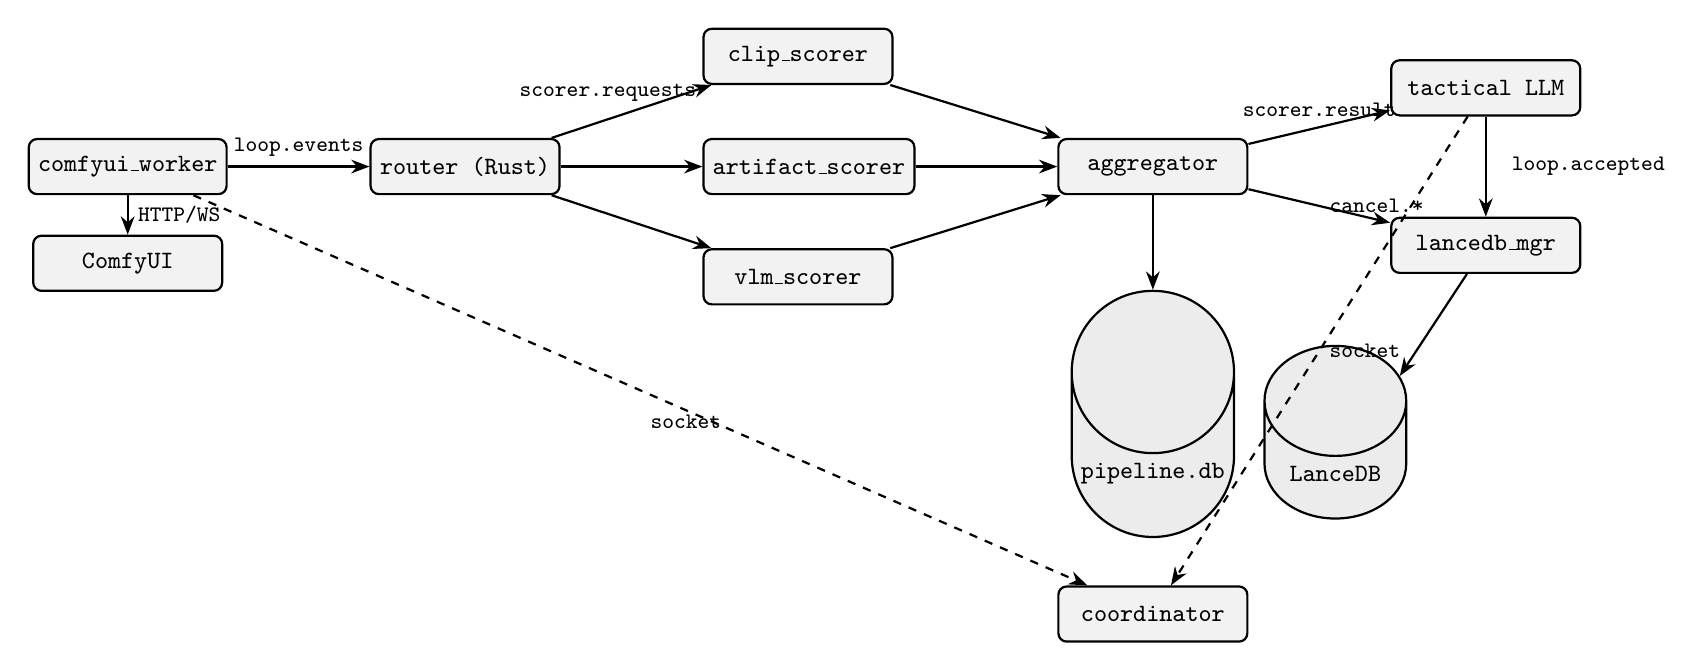
\begin{tikzpicture}[node distance=0.9cm and 1.6cm]
  \node[component] (worker)    {comfyui\_worker};
  \node[component,below=0.5cm of worker] (comfyui) {ComfyUI};
  \node[component,right=1.8cm of worker]  (router)   {router (Rust)};
  \node[component,right=1.8cm of router,yshift=1.4cm]  (clip)     {clip\_scorer};
  \node[component,right=1.8cm of router]               (artifact) {artifact\_scorer};
  \node[component,right=1.8cm of router,yshift=-1.4cm] (vlm)      {vlm\_scorer};
  \node[component,right=1.8cm of artifact] (agg)      {aggregator};
  \node[component,right=1.8cm of agg,yshift=1.0cm]  (tactical) {tactical LLM};
  \node[component,right=1.8cm of agg,yshift=-1.0cm] (ldb)      {lancedb\_mgr};
  \node[store,below=1.2cm of agg]  (sqlite)  {pipeline.db};
  \node[store,right=0.4cm of sqlite] (lancedb) {LanceDB};
  \node[component,below=0.6cm of sqlite] (coord) {coordinator};

  \draw[arrow] (worker)   -- (router)   node[lbl,above] {loop.events};
  \draw[arrow] (router)   -- (clip)     node[lbl,above,xshift=-3mm] {scorer.requests};
  \draw[arrow] (router)   -- (artifact);
  \draw[arrow] (router)   -- (vlm);
  \draw[arrow] (clip)     -- (agg)      node[lbl,above,xshift=3mm] {};
  \draw[arrow] (artifact) -- (agg);
  \draw[arrow] (vlm)      -- (agg);
  \draw[arrow] (agg)      -- (tactical) node[lbl,above] {scorer.result};
  \draw[arrow] (agg)      -- (ldb)      node[lbl,right] {cancel.*};
  \draw[arrow] (tactical) -- (ldb)      node[lbl,right,xshift=2mm] {loop.accepted};
  \draw[arrow] (ldb)      -- (lancedb);
  \draw[arrow] (agg)      -- (sqlite);
  \draw[arrow] (worker)   -- (comfyui)  node[lbl,right] {HTTP/WS};
  \draw[arrow,dashed] (worker)   -- (coord)   node[lbl,right,yshift=-4mm] {socket};
  \draw[arrow,dashed] (tactical) -- (coord)   node[lbl,right] {socket};
\end{tikzpicture}
\end{center}

\section{Address and Queue Topology}

Artemis supports two routing types: \textsc{anycast} (queue semantics, one
consumer receives) and \textsc{multicast} (topic semantics, all subscribers
receive). The table below lists all pipeline addresses.

\begin{center}
\begin{tabular}{lllll}
\toprule
\textbf{Address} & \textbf{Type} & \textbf{Protocol} & \textbf{Publisher} & \textbf{Consumer(s)} \\
\midrule
\texttt{loop.request}          & anycast   & STOMP     & tactical LLM, session & comfyui\_worker \\
\texttt{loop.events}           & multicast & STOMP/AMQP & comfyui\_worker       & router \\
\texttt{scorer.requests}       & multicast & AMQP~1.0  & router                & all scorers \\
\texttt{scorer.events}         & multicast & AMQP~1.0  & aggregator            & all scorers, lancedb\_mgr \\
\texttt{aggregator.clip.queue} & anycast   & STOMP/AMQP & clip\_scorer          & aggregator \\
\texttt{aggregator.artifact.queue} & anycast & STOMP/AMQP & artifact\_scorer    & aggregator \\
\texttt{aggregator.vlm.queue}  & anycast   & STOMP/AMQP & vlm\_scorer           & aggregator \\
\texttt{scorer.result}         & anycast   & AMQP~1.0  & aggregator            & tactical LLM \\
\texttt{loop.accepted}         & multicast & STOMP/AMQP & tactical LLM          & lancedb\_mgr \\
\texttt{tactical.decisions}    & multicast & STOMP     & tactical LLM          & strategic LLM \\
\texttt{pipeline.dead}         & anycast   & AMQP~1.0  & (DLX from all queues) & monitor \\
\bottomrule
\end{tabular}
\end{center}

\section{Data Flow}

\begin{enumerate}
  \item \texttt{session.py} initialises the tactical budget in the coordinator
        via Unix socket (\texttt{BudgetInit}), writes a Session record to
        LanceDB, and publishes the first generation request to
        \texttt{/queue/loop.request} via STOMP.
  \item \texttt{comfyui\_worker} receives the request, registers the image
        session with the coordinator (\texttt{SessionInit}), submits the
        ComfyUI workflow, and waits for completion via WebSocket.
  \item On completion, publishes the result to \texttt{/topic/loop.events}
        via STOMP.
  \item Rust \texttt{router} receives from \texttt{loop.events} via AMQP~1.0
        and fans out to \texttt{scorer.requests} (multicast) with subject
        \texttt{score.<uuid>}.
  \item All three scorers receive the message simultaneously and begin scoring
        in parallel (durable STOMP subscriptions).
  \item As results arrive, the Rust \texttt{aggregator} merges them into the
        \texttt{scorer\_session} SQLite row using \texttt{BEGIN IMMEDIATE}
        transactions.
  \item Threshold evaluation on each arrival:
    \begin{itemize}
      \item CLIP score below threshold: mark rejected in SQLite, publish
            \texttt{cancel.*} to \texttt{scorer.events}, emit rejected verdict
            to \texttt{scorer.result}.
      \item Artifact confidence above threshold: same cancel and reject flow.
      \item All three results within bounds: mark candidate in SQLite, emit
            candidate verdict to \texttt{scorer.result}.
    \end{itemize}
  \item \texttt{tactical\_llm} receives the verdict, queries the coordinator
        for budget state (\texttt{BudgetGet}), retrieves LanceDB session
        history, and runs local LLM inference to decide accept / retry /
        inpaint / give\_up.
  \item On accept: publishes to \texttt{/topic/loop.accepted}. On retry:
        publishes a new request to \texttt{/queue/loop.request} and increments
        the retry counter via \texttt{BudgetUpdate}.
  \item \texttt{lancedb\_manager} receives terminal events (\texttt{loop.accepted}
        or \texttt{cancel.*}), reads the completed \texttt{scorer\_session}
        row, performs an idempotent existence check, and writes the final Loop
        record to LanceDB. The \texttt{scorer\_session} row is deleted after a
        successful write.
\end{enumerate}

\subsection{Cancel Flow}

\begin{center}
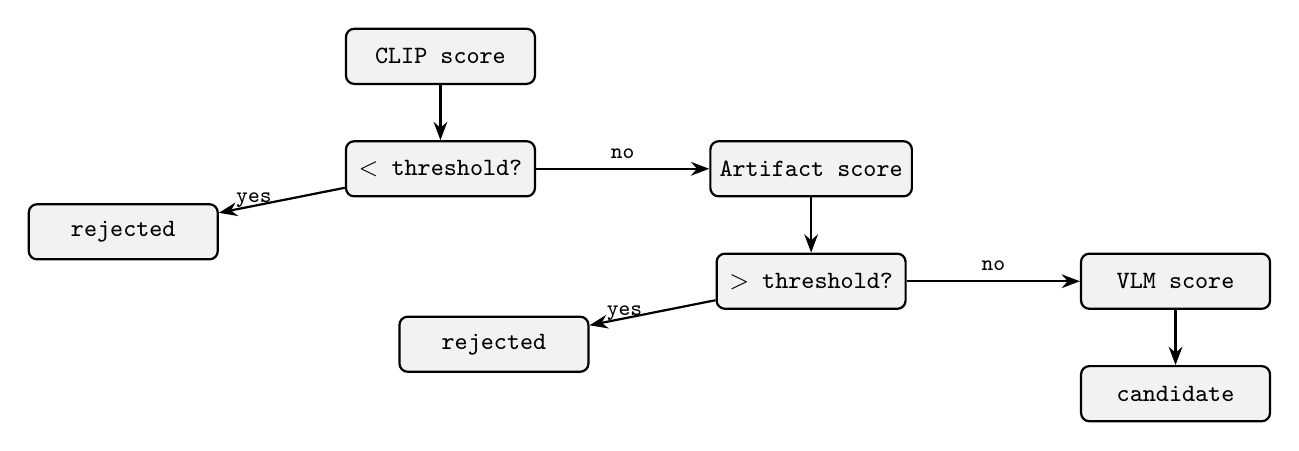
\begin{tikzpicture}[node distance=0.7cm]
  \node[component] (clip) {CLIP score};
  \node[component,below=of clip] (clipcheck) {$<$ threshold?};
  \node[component,right=2.2cm of clipcheck] (artifact) {Artifact score};
  \node[component,below=of artifact] (artcheck) {$>$ threshold?};
  \node[component,right=2.2cm of artcheck] (vlm) {VLM score};
  \node[component,below=of vlm] (candidate) {candidate};
  \node[component,left=1.6cm of clipcheck,yshift=-0.8cm] (r1) {rejected};
  \node[component,left=1.6cm of artcheck,yshift=-0.8cm] (r2) {rejected};

  \draw[arrow] (clip) -- (clipcheck);
  \draw[arrow] (clipcheck) -- node[lbl,above] {no} (artifact);
  \draw[arrow] (clipcheck) -- node[lbl,left] {yes} (r1);
  \draw[arrow] (artifact) -- (artcheck);
  \draw[arrow] (artcheck) -- node[lbl,above] {no} (vlm);
  \draw[arrow] (artcheck) -- node[lbl,left] {yes} (r2);
  \draw[arrow] (vlm) -- (candidate);
\end{tikzpicture}
\end{center}

\section{Persistence Layer}

\subsection{SQLite Operational Database (\texttt{pipeline.db})}

The coordinator owns \texttt{pipeline.db} in WAL mode with
\texttt{PRAGMA synchronous=FULL}. Three tables are defined:

\subsubsection{xa\_log}
Durable XA transaction log for 2-phase commit coordination.

\begin{center}
\begin{tabular}{lll}
\toprule
\textbf{Field} & \textbf{Type} & \textbf{Description} \\
\midrule
\texttt{xid}          & TEXT PRIMARY KEY & Transaction ID \\
\texttt{state}        & TEXT             & prepared $|$ committed $|$ rolledback \\
\texttt{participants} & TEXT             & JSON list of resource managers \\
\texttt{created\_at}  & INTEGER          & Unix timestamp \\
\texttt{resolved\_at} & INTEGER?         & Unix timestamp, null until resolved \\
\bottomrule
\end{tabular}
\end{center}

\subsubsection{scorer\_session}
In-flight per-image state, written by coordinator on \texttt{SessionInit} and
read by aggregator and lancedb\_manager.

\begin{center}
\begin{tabular}{lll}
\toprule
\textbf{Field} & \textbf{Type} & \textbf{Description} \\
\midrule
\texttt{image\_uuid}      & TEXT PRIMARY KEY & Unique per generated image \\
\texttt{session\_uuid}    & TEXT             & Parent session \\
\texttt{sequence\_number} & INTEGER          & Position within session \\
\texttt{prompt}           & TEXT?            & Generation prompt \\
\texttt{workflow\_path}   & TEXT?            & Workflow file path \\
\texttt{workflow\_params} & TEXT?            & JSON generation params \\
\texttt{clip}             & TEXT?            & JSON scorer result, null until arrived \\
\texttt{artifact}         & TEXT?            & JSON scorer result, null until arrived \\
\texttt{vlm}              & TEXT?            & JSON scorer result, null until arrived \\
\texttt{verdict}          & TEXT?            & null $|$ candidate $|$ rejected \\
\texttt{rejection\_reason}& TEXT?            & Rejection cause, null for candidates \\
\texttt{image\_path}      & TEXT?            & Output image URL \\
\texttt{created\_at}      & INTEGER          & Unix timestamp \\
\texttt{expires\_at}      & INTEGER          & Unix timestamp; row deleted by cleanup \\
\bottomrule
\end{tabular}
\end{center}

\subsubsection{tactical\_budget}
Per-session retry and inpaint budget counters.

\begin{center}
\begin{tabular}{lll}
\toprule
\textbf{Field} & \textbf{Type} & \textbf{Description} \\
\midrule
\texttt{session\_uuid}  & TEXT PRIMARY KEY & Session identifier \\
\texttt{retries\_used}  & INTEGER          & Retry attempts consumed \\
\texttt{inpaints\_used} & INTEGER          & Inpaint passes consumed \\
\texttt{max\_retries}   & INTEGER          & Session retry ceiling \\
\texttt{max\_inpaints}  & INTEGER          & Session inpaint ceiling \\
\texttt{created\_at}    & INTEGER          & Unix timestamp \\
\texttt{expires\_at}    & INTEGER          & Unix timestamp (24h TTL) \\
\bottomrule
\end{tabular}
\end{center}

\subsection{Coordinator Unix Socket API}

The coordinator binds a Unix domain socket at
\texttt{\{database.path\}.sock}. Requests and responses are
newline-delimited JSON objects.

\begin{center}
\begin{tabular}{ll}
\toprule
\textbf{Request} & \textbf{Effect} \\
\midrule
\texttt{BudgetInit} & Insert row into \texttt{tactical\_budget} (INSERT OR IGNORE) \\
\texttt{BudgetGet}  & Return budget counters for a session \\
\texttt{BudgetUpdate} & Atomically increment \texttt{retries\_used} or \texttt{inpaints\_used} \\
\texttt{SessionInit}  & Insert row into \texttt{scorer\_session} (INSERT OR IGNORE) \\
\bottomrule
\end{tabular}
\end{center}

\subsection{LanceDB Schema}

\subsubsection{sessions table}
\begin{center}
\begin{tabular}{lll}
\toprule
\textbf{Field} & \textbf{Type} & \textbf{Description} \\
\midrule
\texttt{session\_uuid}   & string      & Primary key \\
\texttt{created\_at}     & string      & ISO 8601 \\
\texttt{user\_prompt}    & string      & Original user prompt \\
\texttt{prompt\_embedding} & vector[512] & CLIP text encoding \\
\bottomrule
\end{tabular}
\end{center}

\subsubsection{loop table}
\begin{center}
\begin{tabular}{lll}
\toprule
\textbf{Field} & \textbf{Type} & \textbf{Description} \\
\midrule
\texttt{image\_uuid}      & string  & Primary key \\
\texttt{session\_uuid}    & string  & FK to sessions \\
\texttt{sequence\_number} & int64   & Position within session \\
\texttt{created\_at}      & string  & ISO 8601 \\
\texttt{prompt}           & string? & Generation prompt \\
\texttt{workflow\_path}   & string? & Workflow file path \\
\texttt{workflow\_params} & string? & JSON generation params \\
\texttt{clip\_score}      & float64? & CLIP similarity \\
\texttt{artifact\_score}  & float64? & AI artifact confidence \\
\texttt{vlm\_photorealism}  & float64? & 0--10 \\
\texttt{vlm\_anatomical}    & float64? & 0--10 \\
\texttt{vlm\_interaction}   & float64? & 0--10 \\
\texttt{vlm\_lighting}      & float64? & 0--10 \\
\texttt{vlm\_prompt}        & float64? & 0--10 \\
\texttt{vlm\_issues}        & string?  & JSON list \\
\texttt{vlm\_recommendations} & string? & JSON list \\
\texttt{verdict}          & string?  & candidate $|$ rejected \\
\texttt{rejection\_reason}& string?  & null for candidates \\
\texttt{image\_path}      & string?  & null for rejected \\
\bottomrule
\end{tabular}
\end{center}

\section{Data-Loss Protection}

\subsection{XA 2-Phase Commit}

The aggregator uses a 2-phase commit protocol coordinated by the coordinator
binary. SQLite serves as the durable XA log with \texttt{PRAGMA
synchronous=FULL}. Phase 1 (Prepare) writes the participant list and fsync
before any phase-2 action. Phase 2 (Commit or Rollback) updates the log entry
and removes the transaction from the in-memory registry.

On startup, the coordinator scans \texttt{xa\_log} for rows in state
\texttt{prepared} and rolls them back (conservative recovery strategy).

\subsection{LanceDB Write Protection}

LanceDB has no XA resource-manager support. Writes are protected by:

\begin{enumerate}
  \item \texttt{scorer\_session} row existence (XA-protected upstream).
  \item Idempotent existence check before each write (\texttt{image\_uuid}
        uniqueness in the \texttt{loop} table).
  \item Message redelivery: ack only after a successful LanceDB write; nack
        without requeue (DLX) on unrecoverable failure.
\end{enumerate}

\subsection{Dead Letter Exchange}

All pipeline queues declare \texttt{x-dead-letter-address: pipeline.dlx}
routing to \texttt{pipeline.dead}. The \texttt{monitor.py} process subscribes
to \texttt{pipeline.dead} and logs all arriving messages for operator review.

\section{Memory Budget}

\begin{center}
\begin{tabular}{lll}
\toprule
\textbf{Component} & \textbf{Role} & \textbf{Memory} \\
\midrule
ComfyUI + SDXL           & Image generation                     & $\sim$14\,GB \\
comfyui\_worker (Python)  & Loop queue consumer                  & $\sim$50\,MB \\
router (Rust)             & Generation event fanout              & $\sim$5\,MB \\
clip\_scorer (Python)     & Prompt adherence + embedding         & $\sim$1.7\,GB \\
artifact\_scorer (Python) & Photorealism scoring                 & $\sim$500\,MB \\
vlm\_scorer (Python)      & Holistic image evaluation            & $\sim$6\,GB \\
aggregator (Rust)         & Result collection and verdict        & $\sim$5\,MB \\
coordinator (Rust)        & XA coordinator + Python budget API   & $\sim$5\,MB \\
lancedb\_manager (Rust)   & LanceDB write manager                & $\sim$5\,MB \\
Tactical LLM (14B Q4)     & Prompt tuning and orchestration      & $\sim$9\,GB \\
ActiveMQ Artemis          & Message broker                       & $\sim$300\,MB \\
OS/UI                     & System overhead                      & $\sim$12\,GB \\
\midrule
\textbf{Total}            &                                      & $\sim$44\,GB \\
\bottomrule
\end{tabular}
\end{center}

Approximately 52\,GB headroom remains in a 96\,GB unified memory system,
leaving room for the VLM scorer ($\sim$6\,GB) running concurrently with a
larger tactical LLM if desired.

\section{Threshold Calibration}

\begin{center}
\begin{tabular}{lll}
\toprule
\textbf{Threshold} & \textbf{Default} & \textbf{Semantics} \\
\midrule
\texttt{thresholds.clip}     & 0.25 & Reject if CLIP score $< 0.25$ \\
\texttt{thresholds.artifact} & 0.50 & Reject if AI confidence $> 0.50$ \\
\bottomrule
\end{tabular}
\end{center}

Both values are placeholders. Calibration procedure:

\begin{enumerate}
  \item Run the loop permissively (\texttt{clip: 0.0}, \texttt{artifact: 1.0}).
  \item Query the \texttt{loop} LanceDB table and examine score distributions.
  \item Set \texttt{clip} at the point below which VLM scores are consistently poor.
  \item Set \texttt{artifact} at the point above which photorealism scores are consistently poor.
  \item Iterate: thresholds too aggressive waste good candidates; too permissive
        waste VLM compute.
\end{enumerate}

All threshold values are read from \texttt{config.yaml} at process startup.
No code changes are required for recalibration.

\section{Scale-Out Path}

\begin{description}
  \item[Multiple ComfyUI workers] Add STOMP consumers on \texttt{/queue/loop.request}.
  \item[Multiple scorer instances] Durable STOMP subscriptions ensure each
        process gets an independent copy of each score request. Add processes;
        no broker reconfiguration needed.
  \item[Remote scoring nodes] Change \texttt{broker.stomp\_url} in
        \texttt{config.yaml}. Artemis handles clustering natively.
  \item[Managed broker] Migrate to Amazon MQ for ActiveMQ (AMQP~1.0 / STOMP
        compatible).
  \item[Cloud LanceDB] Change \texttt{paths.lancedb} to an S3 URI.
\end{description}

\end{document}
